% Copyright 2021 Fausto Spoto
%
% Licensed under the Apache License, Version 2.0 (the "License");
% you may not use this file except in compliance with the License.
% You may obtain a copy of the License at
%
%    http://www.apache.org/licenses/LICENSE-2.0
%
% Unless required by applicable law or agreed to in writing, software
% distributed under the License is distributed on an "AS IS" BASIS,
% WITHOUT WARRANTIES OR CONDITIONS OF ANY KIND, either express or implied.
% See the License for the specific language governing permissions and
% limitations under the License.

\documentclass[11pt]{beamer}  %% versione proiettore
%%\documentclass[11pt,handout]{beamer} %% versione stampa
\usepackage{lucidiJb-2ed}
\usepackage{mathtools}
\usepackage{relsize}
\usepackage[normalem]{ulem}

\mode<article>
{
  \usepackage{fullpage}
  \usepackage{hyperref}
}

\mode<presentation>
{
  \setbeamertemplate{background canvas}[vertical shading][bottom=red!10,top=blue!10]
  \usetheme{Course}
  \usefonttheme[onlysmall]{structurebold}
}

\subtitle{Blockchain Course}
\title{Hotmoka}
\institute{Universit\`a di Verona, Italy}
\date{March 2021}

\setbeamercovered{invisible}

\def\codesize{\smaller}
\def\<#1>{\codeid{#1}}
\newcommand{\codeid}[1]{\ifmmode{\mbox{\codesize\ttfamily{#1}}}\else{\codesize\ttfamily #1}\fi}

\begin{document}

\begin{frame}
  \titlepage
\end{frame}

\begin{frame}
  \frametitle{Hotmoka}

  \begin{greenbox}{\url{https://github.com/Hotmoka/hotmoka}}
    An open-source implementation of a network of nodes:
    \begin{itemize}
    \item nodes of a blockchain
    \item IoT devices
    \item computers in the cloud
    \end{itemize}
  \end{greenbox}

  \bigskip

  \begin{greenbox}{Requests are OO-based}
    \begin{itemize}
    \item create an object
    \item call a method of an object
    \item methods are implemented in a subset of Java
    \end{itemize}
  \end{greenbox}

\end{frame}

\begin{frame}\frametitle{Nodes can be Tendermint applications}

  \begin{center}
    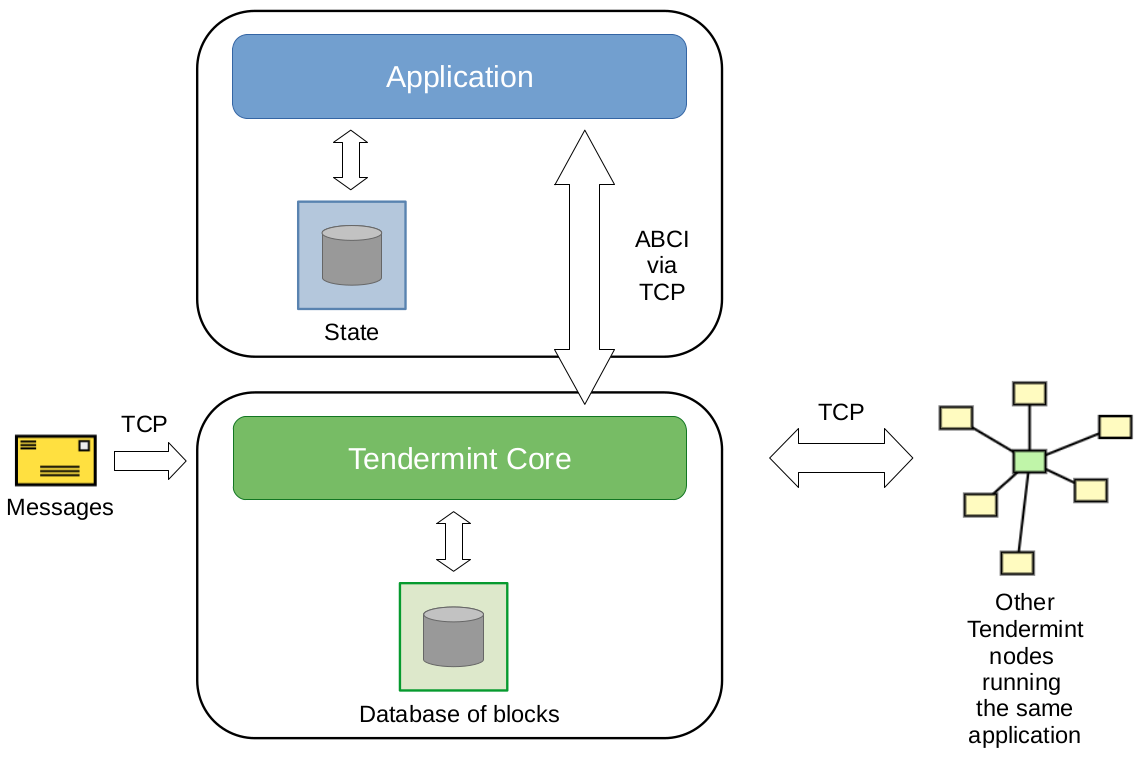
\includegraphics[width=\textwidth,clip=false]{pictures/tendermint-databases.png}
  \end{center}
    
\end{frame}

\begin{frame}\frametitle{The API of a Hotmoka node}

  \begin{itemize}
  \item \<[add|post]JarStore(request):TransactionReference>
  \item \<[add|post]ConstructorCall(request):StorageReference>
  \item \<[add|post|run]InstanceMethodCall(request):StorageValue>
  \item \<[add|post|run]StaticMethodCall(request):StorageValue>
  \item \<subscribeToEvents(key):Subscription>
  \item \<getState(StorageReference):State>
  \end{itemize}

  \bigskip

  \begin{greenbox}{}
    \<add> calls are synchronous (wait for the result)

    \smallskip
    \<post> calls are asynchronous (yield a future)

    \smallskip
    \<run> calls are synchronous and only for read-only methods
  \end{greenbox}

\end{frame}

\begin{frame}\frametitle{An OO state}

  \begin{center}
    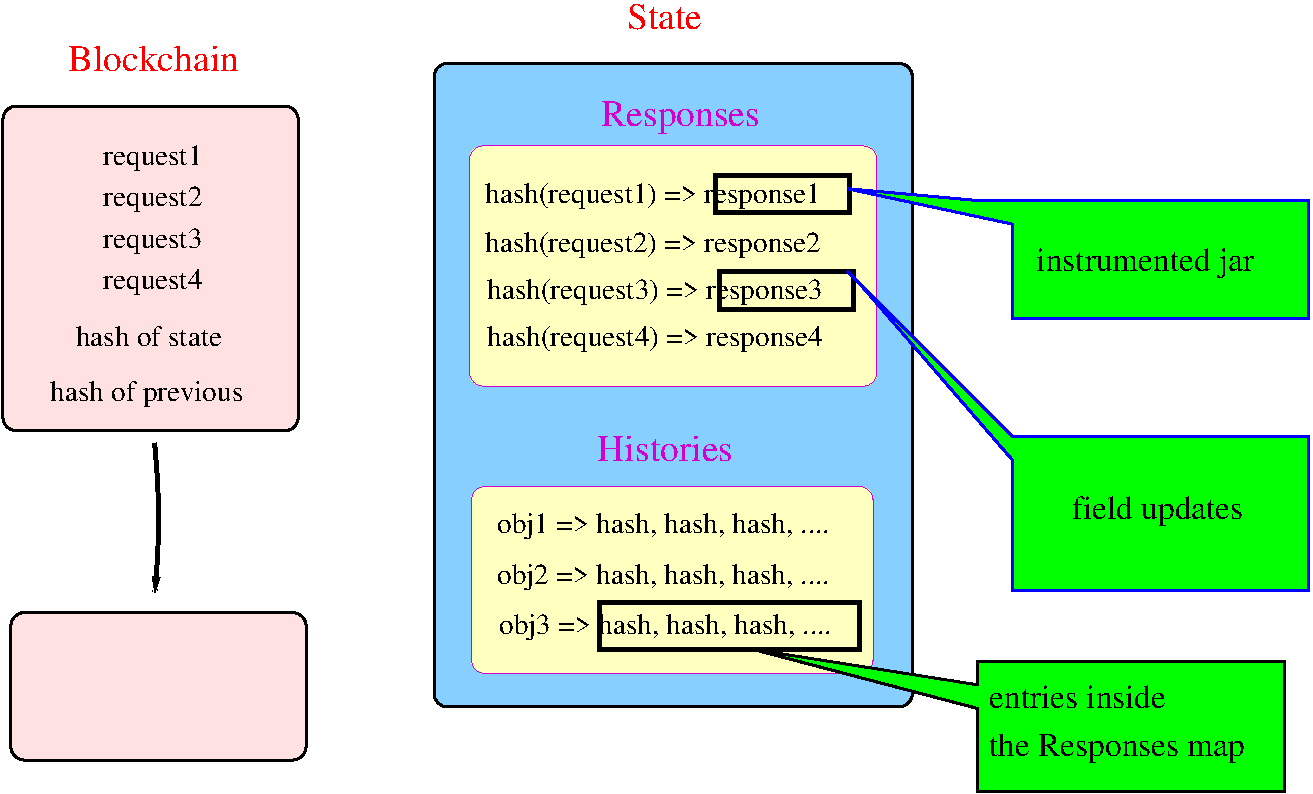
\includegraphics[width=\textwidth,clip=false]{pictures/hotmoka-structure.pdf}
  \end{center}

\end{frame}

\begin{frame}\frametitle{The API of the state}
  
    \begin{enumerate}
    \item get jar at \<hash>: access the Responses map and find the jar
    \item get object at \<obj>: access the Histories at \<obj>: for each \<hash>
      there, access the Responses map at \<hash>, project the updates on \<obj>
      and reconstruct the state of \<obj>
    \item put request/response in state: expand Responses with hash(request)$\Rightarrow$response
      \begin{itemize}
      \item[] if the response contains updates, add hash(request) to the histories of
        the updated objects
      \end{itemize}
    \item \<h=get\_hash()>: compute the hash of the hash of the Merkle-Patricia trie for
      Responses and of that for Histories
    \item \sout{\<checkout(h)>} $\Rightarrow$ unused data from points above are garbage-collected
    \end{enumerate}

\end{frame}

\end{document}
